% =============================================================================
% CRAFT -- reframed manuscript draft (Framing 2 of the adversarial review, sec.20/25)
%
% This is a DRAFT SKELETON written from the revision experiments in ../ .
% Every number carries a source pointer to the script and result file that
% produced it. Numbers marked [PRIOR] are from the previous manuscript and were
% NOT regenerated here -- they must be re-verified before submission.
%
% Build:  pdflatex craft_reframed.tex   (twice, for refs)
% =============================================================================
\documentclass[11pt]{article}

\usepackage[margin=1in]{geometry}
\usepackage{amsmath,amssymb,amsthm}
\usepackage{booktabs}
\usepackage{graphicx}
\usepackage{microtype}
\usepackage[hidelinks]{hyperref}
\usepackage{xcolor}

\newtheorem{lemma}{Lemma}
\newtheorem{proposition}{Proposition}
\newcommand{\eta}{\ensuremath{\eta}}
\newcommand{\src}[1]{{\footnotesize\textcolor{gray}{[\texttt{#1}]}}}
\newcommand{\todo}[1]{\textcolor{red}{\textbf{[TODO: #1]}}}

\title{Compiled Numerical Transformers as a Ground-Truth Testbed:\\
Standard Verification Proxies Give False Reassurance}
\author{\todo{authors}}
\date{\today}

\begin{document}
\maketitle

\begin{abstract}
We compile the triangular solves of LU-based matrix inversion into transformer
weights at binary64 precision, giving a setting in which program structure,
floating-point semantics, and downstream behaviour can all be checked against a
compiler rather than inferred. We use it to ask which of the diagnostics
routinely used to certify that ``a model implements an algorithm'' actually
track program-level correctness. They largely do not. Against compiler-labelled
ground truth, output finiteness reads healthy in $85.7\%$ of runs in which the
attention selector is provably fetching the wrong value; near-zero attention
entropy in $50.0\%$; exact softmax one-hotness in $35.7\%$; and invariance of the
downstream prediction in $9.6\%$. We also give a closed-form
selector-exactness bound that replaces an exhaustive enumeration, extends
validity by four orders of magnitude, and predicts the precision at which
compiled positional addressing fails---at position $11$ in bfloat16, where it
in fact fails. We verify that the compiled program executes genuine run-time
inputs: over $1{,}163$ solves on $40$ matrices with no recompilation, the
per-column normwise backward error never exceeds $1.88\times10^{-16}$ and the
selector hit rate is exactly $1.000$.
\emph{Scope.} The compiler accepts only coefficients known at build time, so no
compiled program in this framework can have input-dependent control flow or
input-dependent coefficients; there is no pivoting. Of the $154$ circuits, $142$
execute the compiled solve and $12$ are direct source reads.
\end{abstract}

% =============================================================================
\section{Introduction}
% =============================================================================

Mechanistic interpretability certifies that a network ``implements an
algorithm'' using diagnostics that are functions of the model's behavioural
surface: attention that is one-hot or low-entropy, outputs that are finite and
plausible, predictions invariant to pruning, individual heads whose ablation is
critical. These are proxies. Whether they track program-level correctness is an
empirical question that cannot be asked without ground truth of a kind that
trained models do not provide.

Compiled models provide it. Tracr \todo{cite} and InterpBench \todo{cite} supply
transformers with known program structure. What they do not supply is a
\emph{floating-point} axis: a setting in which one can perturb precision,
quantization and sparsity and ask, against a compiler, whether the program is
still computing the right numbers. That axis is where the reassurance signals
turn out to fail.

Our contributions:

\begin{enumerate}
\item \textbf{A ground-truth testbed with a floating-point axis} (\S\ref{sec:substrate}):
CRAFT compiles forward/backward substitution for symmetric positive-definite
Laplacian systems into transformer weights, at binary64, with every dimension's
role known before execution.
\item \textbf{The main result} (\S\ref{sec:main}): a measured dissociation between
four standard behavioural proxies and compiler-labelled correctness, with
false-reassurance rates and cluster-bootstrap intervals.
\item \textbf{A precision-requirement characterization} (\S\ref{sec:mechanism}):
a closed-form margin condition for exact hard-attention positional addressing,
giving a design rule for any (encoding, position range, precision) triple. The
selector scale $K$ cancels---a result that falsifies the mechanism we ourselves
previously proposed for quantization failure.
\item \textbf{An honest downstream accounting} (\S\ref{sec:readout}): the
application-level voltage metric is a quantization budget, not an accuracy
result, and we decompose it rather than reporting a pass count.
\end{enumerate}

We deliberately do \emph{not} claim that CRAFT is a useful solver. It is roughly
five orders of magnitude slower than \texttt{numpy.linalg.solve}. It is an
instrument, and the point of an instrument is inspectability.

% =============================================================================
\section{The CRAFT substrate}\label{sec:substrate}
% =============================================================================

\paragraph{What is compiled and what is not.} The host computes the Doolittle
factors $\hat L,\hat U$ of $A_{FF}$ once at build time; these are baked into
token embeddings. The transformer executes the remaining forward and backward
substitution, token by token. A runner mediates the KV cache between steps,
supplying $b_i$ at \texttt{rhs}$_i$ and $y_i$ at \texttt{bck}$_i$. Table
\ref{tab:ownership} states the boundary; nothing in this paper claims the
factorization itself is executed by the network.

\paragraph{The hard ceiling.} The compiler accepts only coefficients known at
build time. Consequently no compiled program here can express pivoting,
input-dependent control flow, or input-dependent coefficients, and each matrix
requires its own compilation at $O(n^4)$ cost. This is a boundary of the
framework, not a defect of an implementation, and it determines what ``a
transformer executes a numerical routine'' can mean in this setting.

\begin{table}[t]
\centering
\caption{Ownership. \todo{port Table 6 from the prior manuscript}}
\label{tab:ownership}
\begin{tabular}{lll}
\toprule
Stage & Owner & Evidence \\
\midrule
$A$ assembly, $LU$ factorization & host (build time) & --- \\
forward/backward substitution & transformer & \S\ref{sec:runtime} \\
value threading between steps & runner & \S\ref{sec:runtime} \\
\bottomrule
\end{tabular}
\end{table}

\paragraph{Two populations.} Of the $154$ circuits, the target node is a
\emph{fixed} (source) node in $12$. For those the compiler emits a direct source
read: the substitution machinery is compiled and scheduled but never exercised,
and $88$ free-variable solve steps are built and never run. These circuits attain
zero downstream error without executing a solve. \textbf{Every execution claim in
this paper is reported on the $142$ circuits that execute the solve}, and the
$12$ are reported separately.
\src{revision/p01\_runtime\_rhs.py}

% =============================================================================
\section{The instrument executes run-time inputs}\label{sec:runtime}
% =============================================================================

A compiled program whose only exercised input is a column of the identity cannot
be distinguished from a constant emitter. We therefore drive each compiled model
with six families of right-hand side, \emph{with no recompilation between them}.

\begin{table}[t]
\centering
\caption{Run-time right-hand-side generalization. $40$ matrices, $1{,}163$
solves, no recompilation. $u = 1.11\times10^{-16}$. Statistical unit is the
(matrix, right-hand side) pair; we report per-family maxima.}
\label{tab:runtime}
\small
\begin{tabular}{lrrrr}
\toprule
RHS family & $n$ & $\max \eta$ & median $\eta$ & selector hit \\
\midrule
identity columns $e_j$        & 243 & $1.58\times10^{-16}$ & $1.25\times10^{-17}$ & $1.000$ \\
source-driven (physical $b$)  &  40 & $1.88\times10^{-16}$ & $4.16\times10^{-17}$ & $1.000$ \\
i.i.d.\ Gaussian              & 400 & $1.64\times10^{-16}$ & $1.44\times10^{-17}$ & $1.000$ \\
wide dynamic range ($10^{-8}$--$10^{8}$) & 400 & $1.78\times10^{-16}$ & $2.11\times10^{-17}$ & $1.000$ \\
all-ones Poisson forcing, \emph{in-model} & 40 & $1.09\times10^{-16}$ & $1.36\times10^{-17}$ & $1.000$ \\
adversarial (min.\ singular direction) & 40 & $1.18\times10^{-16}$ & $1.19\times10^{-17}$ & $1.000$ \\
\bottomrule
\end{tabular}
\src{revision/p01\_runtime\_rhs.py $\to$ results/p01\_summary.json}
\end{table}

Table \ref{tab:runtime} shows the error on arbitrary run-time input is
indistinguishable from the error on identity columns, with max-of-max
$\eta = 1.88\times10^{-16} \approx 1.7u$ and a selector hit rate against the
compiler-labelled float64 trace of exactly $1.000$ throughout. The instrument
solves; it does not replay.

\paragraph{Numerical calibration, not a finding.} The measured
$\eta = O(u)$ is what classical theory predicts. Theorem 2 of the prior
manuscript is the Rigal--Gaches (1967) normwise backward-error theorem
\todo{cite}, Higham Thm 7.1 \todo{cite}, with Oettli--Prager (1964) as the
componentwise ancestor; we instantiate it, we do not extend it. With a measured
growth factor $\|\hat L\|\|\hat U\|/\|A\| = 1.2$ \textsc{[prior]}, classical LU
stability theory \todo{cite Higham Ch.~8--9} predicts $\eta = O(u)$ with small
constants, and that is what we observe. We report this as calibration of the
instrument.

% =============================================================================
\section{Main result: proxies dissociate from correctness}\label{sec:main}
% =============================================================================

\paragraph{Ground truth.} A run is \emph{broken} when any attention lookup
fetches from a position other than the one the compiler scheduled, as directly
observed in the float64 production trace, or when the output is not finite. We
deliberately do not label float32 broken merely for attaining $\eta \approx
u_{f32}$: executing the same program correctly in lower precision is a different
thing from executing the wrong program. This makes the negative result harder to
obtain, not easier.

\paragraph{Proxies.} A proxy reads \emph{green} for a configuration when its
value is no worse than the float64 reference on the same matrix. Absolute
thresholds are degenerate here: requiring every lookup in a run to be exactly
one-hot is not satisfied even by provably correct runs. Attention entropy is the
true Shannon entropy, computed \emph{without} the $10^{-30}$ regulariser that
produced the $10^{-28}$-nat artifacts we previously reported and disowned.

\paragraph{Grid.} Selector scale $K\in\{10^{10},10^{8},10^{6},10^{4}\}$ $\times$
dtype $\{$f64, f32, bf16, f16$\}$ $\times$ quantization $\{$none, per-tensor
int8, per-channel int8$\}$ $\times$ pruning $\{0,10,50,90\%\}$, computed both
over all coefficients and over nonzero coefficients only. $10$ matrices,
$480$ cells, $280$ broken.

\begin{table}[t]
\centering
\caption{False-reassurance rates. Statistical unit is the (matrix,
configuration) cell; intervals are cluster bootstraps over matrices.}
\label{tab:proxies}
\small
\begin{tabular}{lrrr}
\toprule
Behavioural proxy & green on correct runs & $P(\text{green}\mid\text{broken})$ & 95\% CI \\
\midrule
outputs all finite                & $100.0\%$ & $\mathbf{85.7\%}$ & $[86, 86]$ \\
attention entropy                 & $80.0\%$  & $\mathbf{50.0\%}$ & $[46, 54]$ \\
softmax one-hot fraction          & $100.0\%$ & $\mathbf{35.7\%}$ & $[31, 40]$ \\
prediction unchanged (50\,mV grid) & $100.0\%$ & $\mathbf{9.6\%}$  & $[0, 27]$ \\
\midrule
all four simultaneously           & ---       & $2.9\%$ (8/280)   & --- \\
\bottomrule
\end{tabular}
\src{revision/p11b\_analyze\_and\_figure.py $\to$ results/p11\_diagnosticity.json}
\end{table}

\begin{figure}[t]
\centering
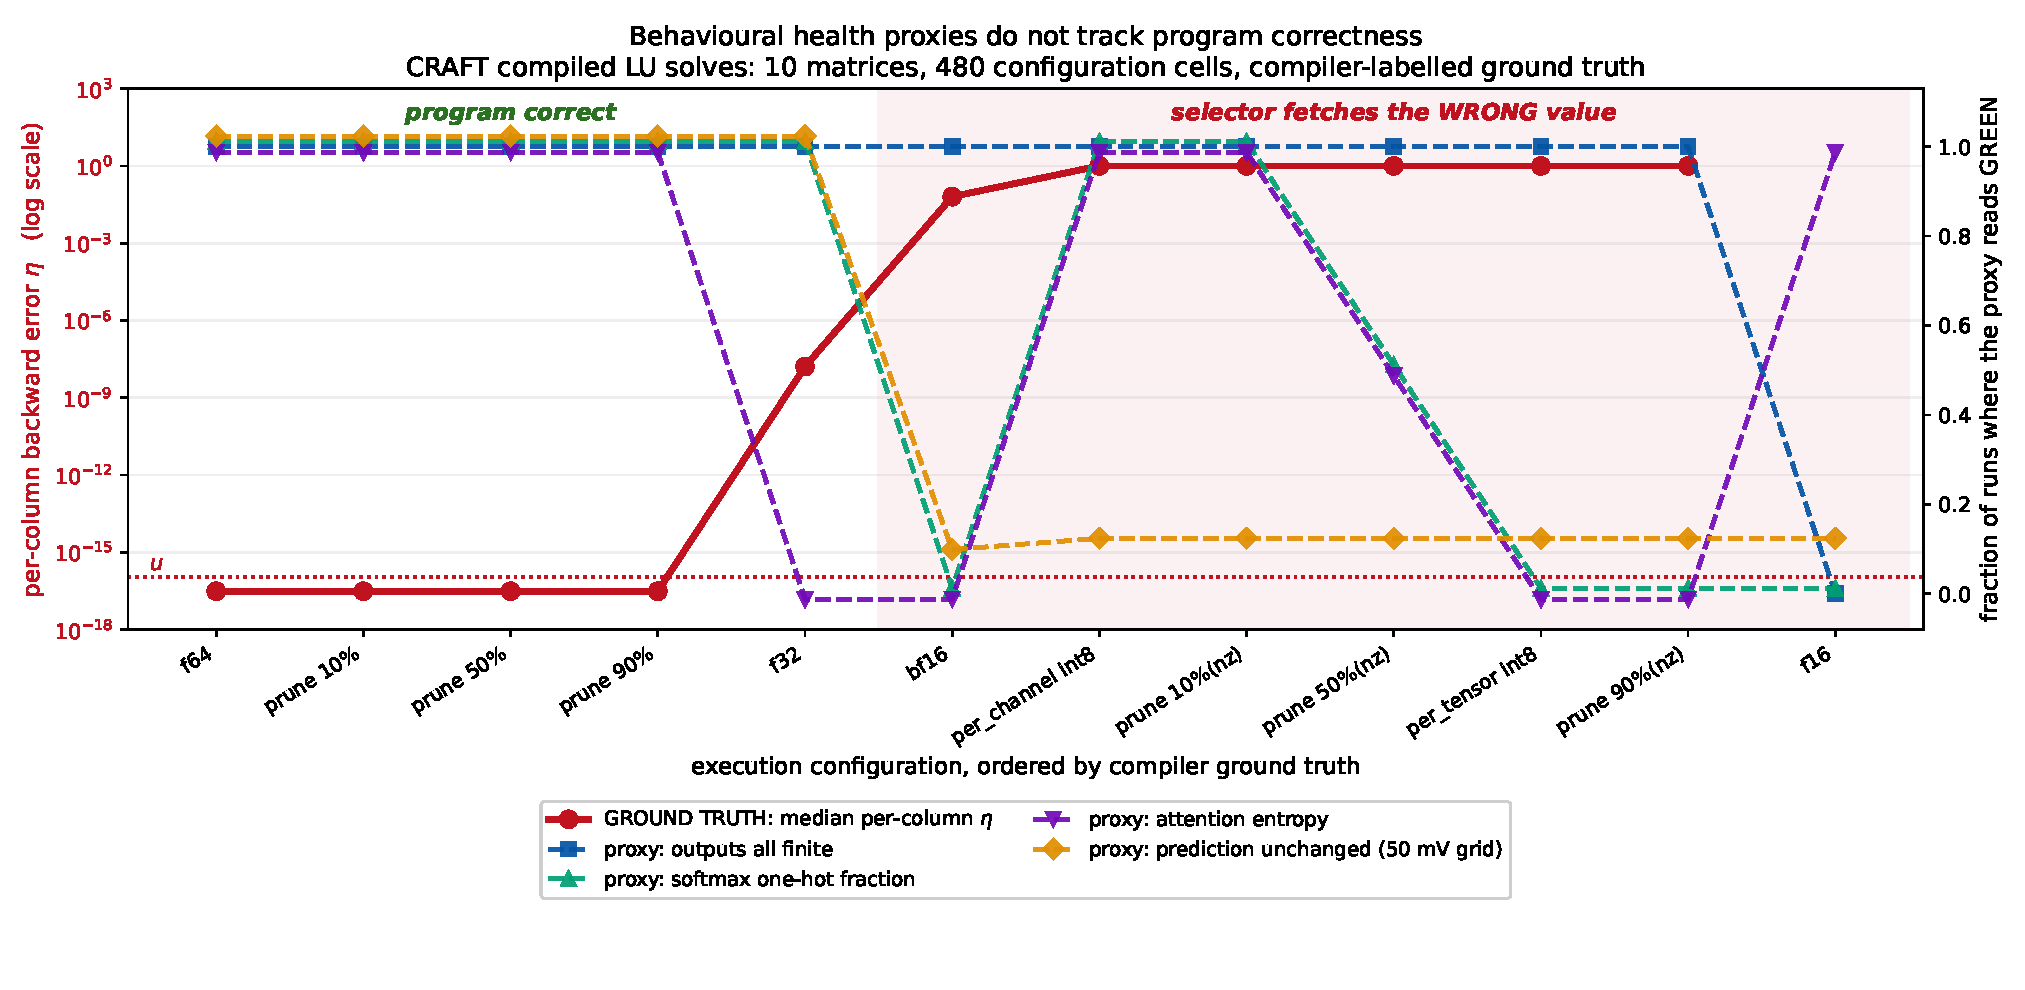
\includegraphics[width=\textwidth]{killer_figure.pdf}
\caption{Behavioural health proxies do not track program correctness.
Configurations are ordered by compiler ground truth. The ground-truth curve
(red, left axis) rises fifteen orders of magnitude while the proxy curves
(right axis) stay flat near $1.0$ across a substantial part of the range.}
\label{fig:killer}
\end{figure}

\paragraph{Pruning invariance is structural sparsity.} Pruning $10/50/90\%$ of
\emph{all} coefficients leaves execution bit-identical
($\eta = 3.07\times10^{-17}$, hit rate $1.000$). Pruning $10\%$ of the
\emph{nonzero} coefficients destroys it ($\eta = 1.00$, hit rate $0.915$). Our
previous $90\%$-pruning-invariance result measured the sparsity of the compiled
weight tensor, not robustness. Restated over nonzero coefficients it becomes a
further instance of the dissociation above.

% =============================================================================
\section{Mechanism: a precision requirement, not a scale pathology}\label{sec:mechanism}
% =============================================================================

With parabolic positional keys $k_p = \tfrac{K}{\sqrt2}(2p,\, -p^2 + \alpha g(p))$
and query $q_t = \tfrac{K}{\sqrt2}(t,\,1)$, the post-max-subtraction score is
$s(p) = -\tfrac{K}{2}(t-p)^2 + \tfrac{K}{2}\alpha g(p)$, maximised uniquely at
$p=t$.

\begin{lemma}[Selector exactness]\label{lem:margin}
With $0 \le g < 1/\ln 2$ and $\alpha < \ln 2$, the exact score gap to the nearest
competitor is at least $1 - \alpha/\ln 2$ in units of $K/2$. The computed argmax
is exact, and the softmax exactly one-hot after max-subtraction and underflow,
whenever
\[
1 - \frac{\alpha}{\ln 2} \;>\; c\,\varepsilon\,t^{2},
\]
where $\varepsilon$ is the unit roundoff of the execution format and $c$ counts
the accumulated terms. The selector scale $K$ cancels from both sides.
\end{lemma}

\begin{table}[t]
\centering
\caption{The bound as a design rule, with $\alpha = 0.3$
($1-\alpha/\ln 2 = 0.5672$; the true minimum gap over $t\in[1,2\times10^5]$ is
$0.9996$).}
\label{tab:margin}
\small
\begin{tabular}{lrr}
\toprule
precision & closed-form $t_{\max}$ & empirical first failure \\
\midrule
float64  & $3.57\times10^{7}$ & none up to $4\times10^{6}$ \\
float32  & $1.54\times10^{3}$ & $5{,}650$ \\
bfloat16 & $6.0$              & $\mathbf{11}$ \\
float16  & $17.0$             & $1$ (overflow, not precision) \\
\bottomrule
\end{tabular}
\src{revision/p02\_margin\_bound.py $\to$ results/p02\_margin\_bound.json}
\end{table}

Lemma \ref{lem:margin} replaces the $361{,}201$-pair enumeration through
$p \le 601$ of the prior manuscript; that ceiling was an artifact of exhaustive
checking, and the bound licenses four orders of magnitude beyond it. It also
\emph{predicts} the bfloat16 failure position, which is where it occurs
(Table \ref{tab:margin}). This is the deliverable for anyone writing constructive
transformer results that assume real arithmetic: given a positional encoding and
a position range, it says what precision suffices.

\paragraph{A mechanism we previously asserted is false.} We previously explained
the int8 collapse by saying the $10^{10}$ selector coefficient set the tensor
scale and rounded the arithmetic coefficients away. Varying $K$ over six orders
of magnitude changes nothing: per-tensor int8 hit rate moves from $0.898$
($K=10^{10}$) to $0.903$ ($K=10^{4}$) with $\eta = 1.00$ throughout, and
bfloat16 $\eta$ stays at $5$--$7\times10^{-2}$. Per-channel int8, the scheme we
cited but had not run, improves the hit rate to $0.924$ and does not restore
execution. Consistently, $K$ cancels from Lemma \ref{lem:margin}: $K=10^{10}$
buys no exactness and is a pure overflow and quantization liability.
\src{revision/p11\_proxy\_diagnosticity.py}

% =============================================================================
\section{The downstream readout is a quantization budget}\label{sec:readout}
% =============================================================================

The application-level metric of the prior manuscript---fraction of circuits whose
predicted node voltage falls within $50$\,mV---cannot distinguish solvers. With
bin width $h = 50$\,mV the quantization ceiling is $h/2 = 25$\,mV and the
uniform-in-bin expectation is $h/4 = 12.5$\,mV.

\begin{table}[t]
\centering
\caption{Three-way error decomposition over all $154$ circuits.}
\label{tab:voltage}
\small
\begin{tabular}{lrr}
\toprule
component & mean & max \\
\midrule
\textbf{total error} & $\mathbf{11.84}$\,mV & $50.00$\,mV \\
readout quantization & $11.84$\,mV & $50.00$\,mV \\
SPICE-vs-Laplacian target mismatch & $0.0246$\,mV & $0.0494$\,mV \\
\textbf{the solve itself} & $\mathbf{1.6\times10^{-10}}$\,mV & $8.7\times10^{-9}$\,mV \\
\bottomrule
\end{tabular}
\src{revision/p05\_voltage\_decomposition.py $\to$ results/p05\_summary.json}
\end{table}

Total error equals quantization error to four significant figures; the solve
contributes eleven orders of magnitude less than the metric's resolution.
$99.35\%$ of circuits fall within the $25$\,mV ceiling and nothing lies between
$25$ and $50$\,mV. One circuit sits at $50.00000000000071$\,mV, which is why we
report an error CDF rather than a pass count at a threshold. We also report the
statistic for the $\max(s,0)$ clamp that the pipeline applies: $0$ of $1{,}437$
solution entries across all $154$ circuits are negative, so the clamp is a
provable no-op on the declared domain.

% =============================================================================
\section{Systems appendix: exact sub-linear selector lookup}\label{sec:hull}
% =============================================================================

Attention lookup here is $2$-D maximum inner product search, and the Hull cache
is the dynamic convex hull trick \todo{cite Overmars--van Leeuwen,
Brodal--Jacob, Li Chao} applied to it. Timed against a \emph{fair} baseline---a
batched \texttt{argmax}$(Kq)$ over a preallocated contiguous buffer, same
process, same language, same float64 keys, fused insert-and-query:

\begin{table}[t]
\centering
\caption{Per-query microseconds, single-threaded, one process.}
\label{tab:hull}
\small
\begin{tabular}{lrrrr}
\toprule
$L$ & shipped cache & dense loop & dense batched & Hull (C++) \\
\midrule
$100$     & $31.7$    & $22.0$   & $\mathbf{1.45}$   & $7.89$ \\
$1{,}000$ & $154.9$   & $50.4$   & $14.82$           & $\mathbf{8.31}$ \\
$10{,}000$& $1428.3$  & $271.8$  & $172.86$          & $\mathbf{11.34}$ \\
$100{,}000$& ---      & $2846.6$ & $1937.52$         & $\mathbf{16.13}$ \\
\bottomrule
\end{tabular}
\src{revision/p03\_hull\_fair\_baseline.py}
\end{table}

The $O(\log L)$ behaviour is real---per-query cost moves from $7.9$ to
$16.1\,\mu$s across a $1000\times$ increase in $L$---with a crossover at
$L \approx 600$. But the $55\times$ figure of the prior manuscript is not
defensible: against the fair baseline the speedup at $L=10{,}000$ is
$15.2\times$, and the shipped cache was $8.3\times$ slower than a batched dense
argmax at the same length for reasons of language and access pattern.

% =============================================================================
\section{Limitations}\label{sec:limitations}
% =============================================================================

\begin{itemize}
\item \textbf{Build-time coefficients only.} No pivoting, no input-dependent
control flow, no input-dependent coefficients. This is a ceiling on the
framework.
\item \textbf{Scale.} All executed systems have $\le 44$ unknowns. Schedules are
generated to $n=200$ but not executed at that size here.
\item \textbf{Reduction order depends on a MILP solve.} Compiling one circuit
under five solver configurations (HiGHS seeds $0/1/7$, a reduced time limit, and
CBC) yields five distinct weight files in every case, and for one of four
circuits tested the \emph{executed result changes bits} ($1.84$ ulp, traceable to
a third distinct slot map and hence a different reduction order). Bitwise
reproducibility claims must be scoped to a fixed schedule.
\src{revision/p07\_schedule\_stability.py}
\item \textbf{One compiler, one architecture family.} No cross-architecture claim
is possible.
\item \textbf{Explicit inversion.} Forming $\hat X$ and multiplying is the
classical antipattern \todo{cite Higham Ch.~14}; it is the source of the $O(n^4)$
cost and of the need for per-column rather than single certificates.
\item \textbf{Not a solver.} Roughly $10^5\times$ slower than
\texttt{numpy.linalg.solve}.
\item \textbf{Domain.} Grounded Laplacians and generated Poisson stencils. The
$567$ ``external'' targets are produced by our own converter, which discards
diagonals and signs; that is a sparsity-pattern sweep, not a domain shift, and is
renamed accordingly.
\end{itemize}

% =============================================================================
\section*{Reproducibility}
% =============================================================================

All results in \S\ref{sec:runtime}--\S\ref{sec:hull} are produced by the scripts
in \texttt{revision/}, on CPU in float64, under one pinned source tree; see
\texttt{revision/README.md}. \todo{P0.8: every reference in this paper must be
independently verified to exist before submission. The prior bibliography
contained multiple 2026-dated arXiv entries alongside a disclosure of
LLM-assisted literature search, and no citation here should be trusted until
checked against a canonical source.}

\todo{Add missing prior art: Rigal--Gaches; Oettli--Prager; Higham Ch.~8--9, 14;
Graves et al.\ NTM/DNC for the runner-plus-memory architecture; Overmars--van
Leeuwen and Brodal--Jacob for dynamic planar convex hull; attention-as-MIPS;
Hahn 2020, P\'erez et al., Merrill \& Sabharwal on hard-attention expressivity;
INTLAB/\texttt{verifylss}, Ogita--Rump--Oishi, Flocq/Gappa for verified numerics;
quantized-iteration limit cycles.}

\bibliographystyle{plain}
% \bibliography{craft}

\end{document}
